% Ajustar esse \vspace de acordo com o necessário
\vspace{-42pt}
Teste de citação: \cite{DepEngEle}
Na parte de hardware, teremos que utilizar:
\begin{itemize}
   \item O servidor do LCEE que fará a armazenagem e processamento de dados; 
   \item Um leitor de RFID para registrar o login do usuário;
   \item Arduíno para viabilizar a comunicação do leitor RFID com o servidor;
   \item Tranca eletrônica para segurança dos equipamentos/KITs.
\end{itemize}
Já na parte de software podemos utilizar:
\begin{itemize}
   \item Um Framework PHP como o Laravel ou CakePHP para facilitar no desenvolvimento do sistema de login; 
   \item Banco de dados SQL (Structured Query Language).
\end{itemize}

Uma inspiração que temos para software é a plataforma web Lend-Itens. Abaixo podemos ver como ficará a plataforma Web:

\begin{figure}[!h]
	\centering
	\caption{Na plataforma Lend-Itens, os usuários podem acessar sua biblioteca para pesquisar um item e reservá-lo, bem como ver seu histórico e os empréstimos atuais.}
	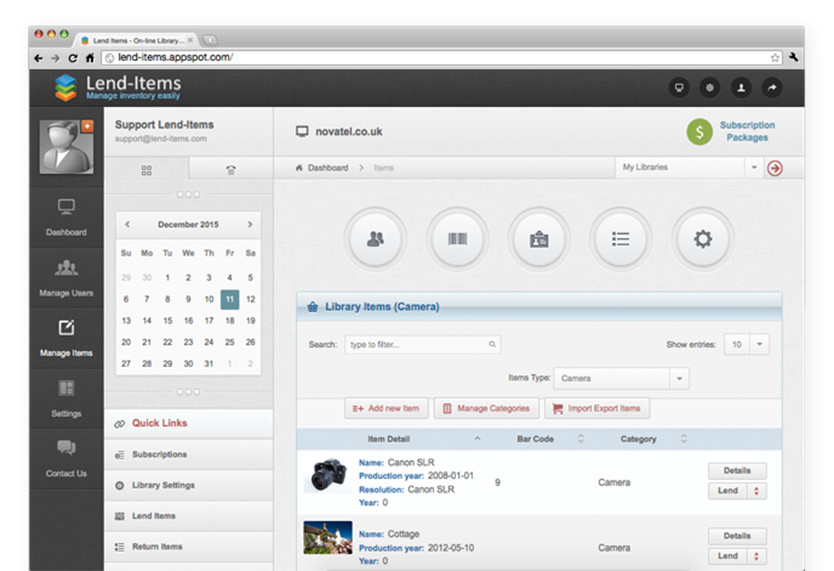
\includegraphics[width=0.7\textwidth]{figura1.jpg}
	\source[\citeonline{DepEngEle}.]
	\label{fig:label_da_figura}
\end{figure}

\begin{figure}[!h]
	\centering
	\caption{Pode-se verificar quais são as pessoas que utilizam a plataforma.}
	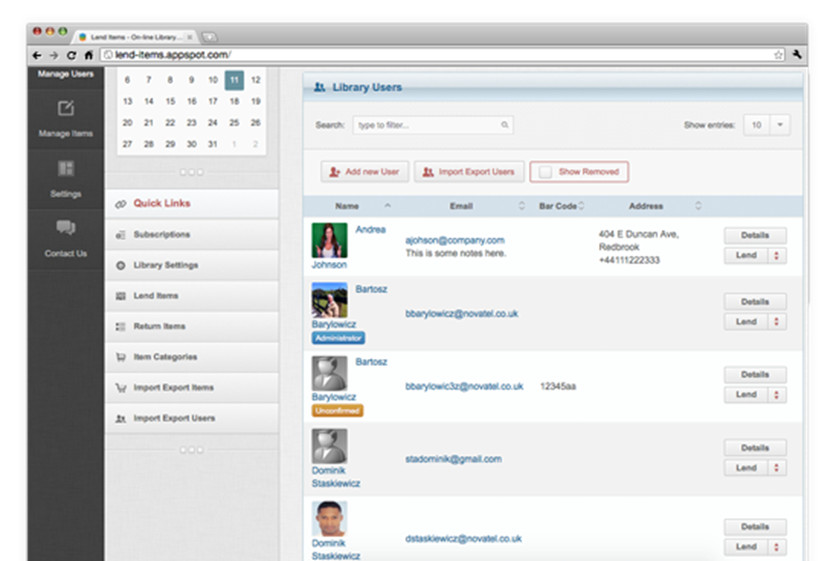
\includegraphics[width=0.7\textwidth]{figura2.jpg}
	\source[\citeonline{DepEngEle}.]
	\label{fig:label_da_figura}
\end{figure}

Outras plataformas que podemos ter como base são Vaivem, apresentando a seguinte interface:

\begin{figure}[!h]
	\centering
	\caption{Interface de Vaivem.}
	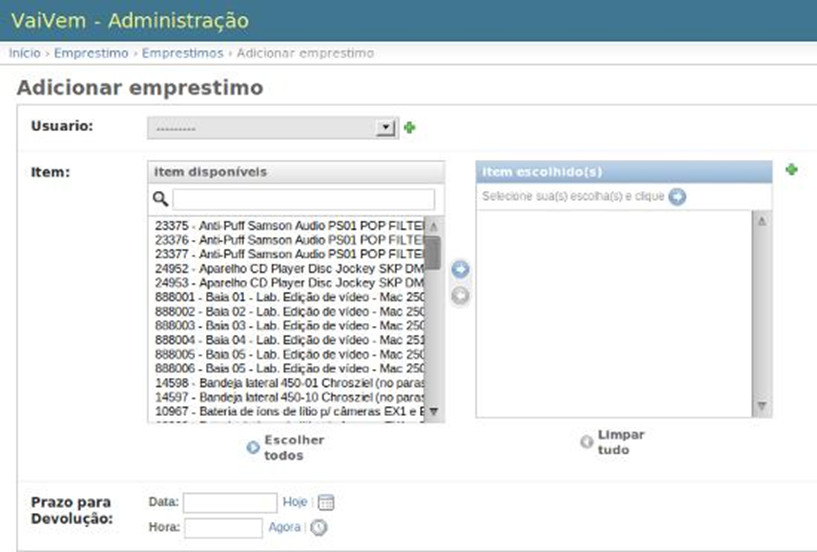
\includegraphics[width=0.7\textwidth]{figura3.jpg}
	\source[\citeonline{DepEngEle}.]
	\label{fig:label_da_figura}
\end{figure}


Há outros softwares também como Software de Controle de UPJ e TotalLoc.
Também estamos utilizando o seguinte modelo de banco de dados para nosso projeto :
\begin{figure}[!h]
	\centering
	\caption{Configuração do Banco de Dados.}
	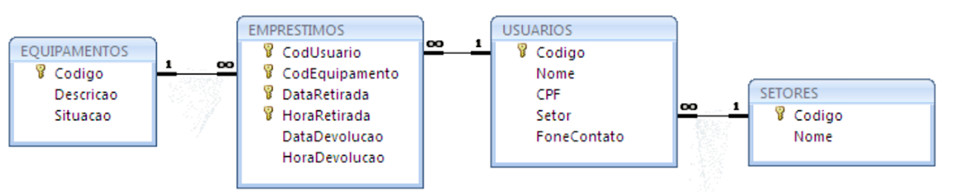
\includegraphics[width=0.7\textwidth]{figura4.jpg}
	\source[\citeonline{DepEngEle}.]
	\label{fig:label_da_figura}
\end{figure}


Também podemos ver quando o banco é acessado pelo seguintes esquemático:

\begin{figure}[!h]
	\centering
	\caption{Acesso do Banco de Dados.}
	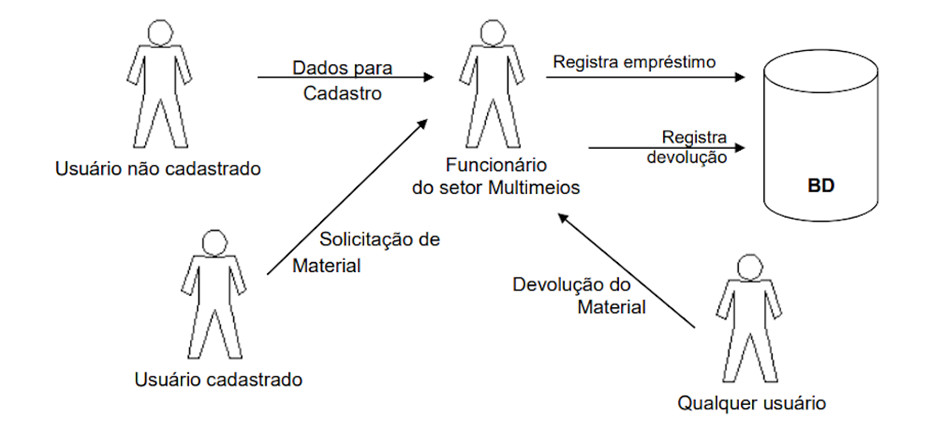
\includegraphics[width=0.7\textwidth]{figura5.jpg}
	\source[\citeonline{DepEngEle}.]
	\label{fig:label_da_figura}
\end{figure}
